%\subsection{Подход М.М.Ботвинника}
\begin{frame}{Подход М.М.Ботвинника}
Ботвинник предлагал анализировать расположение фигур на статической доске. Для этого необходимо: 
\begin{itemize}
\item определить локальные цели для данной позиции;
\item наметить план достижения цели;
\item проверить осуществимость плана;
\item предусмотреть действия противника;
\item объединить все планы в единое представление позиции;
\item определить оптимальную последовательность действий.
\end{itemize}
Данный подход рассматривался как средство решения широкого класса комбинаторно-оптимизационных задач.
\end{frame}

%\subsection{Основные понятия}
\begin{frame}{Основные понятия}
\begin{description}
\item[Траектория] последовательность полей движения фигуры на пустой доске
\item[Горизонт] максимальная длина рассматриваемых траекторий
\item[Цель] фигуры противника или поля
\item[Подцепочка] действия, направленные на достижение цели
\item[Цепочка] совокупность действий, направленных на достижение цели
\item[Вилочность] совпадение частей цепочек
\item[Оценка фигуры] числовая характеристика <<полезности>> фигуры
\item[Время успевания] допустимое число ходов для защиты от атаки противника
\end{description}
\end{frame}

\begin{frame}{Цепочка~--- ключевое понятие метода}
\begin{columns}
\column{0.5\textwidth}
\begin{figure}[t]
  \only<1>{\scalebox{0.8}{\showDiagram{Pa5, Na7, bh3}{a5-a8}}}
  \only<2>{\scalebox{0.8}{\showDiagram{Pa5, Na7, bh3}{a7-b5, a7-c8, a7-c6}}}
  \only<3>{\scalebox{0.8}{\showDiagram{Pa5, Na7, bh3}{h3-g2, g2-a8}}}
  \only<4>{\scalebox{0.8}{\showDiagram{Pa5, Na7, bh3}{a7-b5,b5-c7}}}%, a7-c8-b6-a8}}}
  \only<5>{\scalebox{0.8}{\showDiagram{Pa5, Na7, bh3}{a7-b5}}}%, a7-c8-b6-a8}}}
\end{figure}
\column{0.5\textwidth}
\textbf{Цель} - достижение пешкой поля a8 \\
\textbf{Траектория} - \alert<1>{a5-a6-a7-a8} \\
\pause
\textbf{Подцепочка-1} - освобождение траектории \alert<2,5>{a7-b5}\alert<2>{, a7-c6, a7-c8} \\
\pause
\textbf{Подцепочка-1} - защита противника \alert<3>{h3-g2-(a8)}, h3-f1-(a6), h3-c8-(a6) \\
\pause
\textbf{Подцепочка-2} - поддержка \alert<4,5>{a7-b5}\alert<4>{-c7-(a8, a6)}, a7-c8-b6-(a8) (защита от подцепочки-1)
\pause
\textbf{Вилочность} - освобождение + поддержка
\end{columns}
\end{frame}

\begin{frame}{Пример цепочки: дерево}
\begin{tabular}{ll}
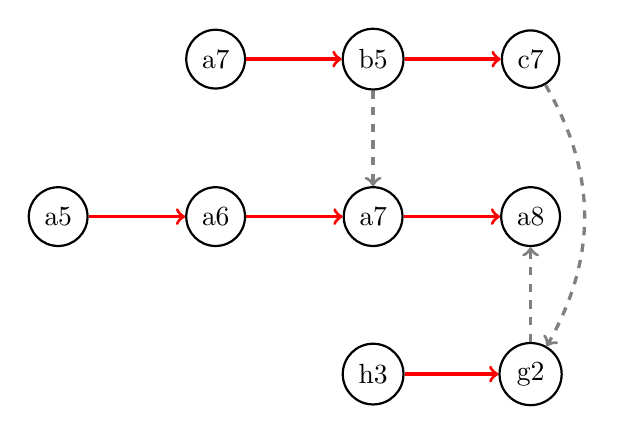
\begin{tikzpicture}
\begin{scope}[every node/.style={circle,thick,draw}]
    \node (A5) at (0,0) {a5};
    \node (A6) at (2,0) {a6};
    \node (A7) at (4,0) {a7};
    \node (A8) at (6,0) {a8};
    \node (NA7) at (2,2) {a7};
    \node (B5) at (4,2) {b5};
    \node (C7) at (6,2) {c7};
    \node (H3) at (4,-2) {h3};
    \node (G2) at (6,-2) {g2};
\end{scope}

\begin{scope}[%>={Stealth[black]},
              every node/.style={fill=white,circle},
              every edge/.style={draw=red,very thick}]
    % подцепочка 0
    \path [->] (A5) edge (A6);
    \path [->] (A6) edge (A7);
    \path [->] (A7) edge (A8);
    % Защита
    \path [->] (H3) edge (G2);
    \path [->] (G2) edge[gray, draw=gray, dashed] (A8);
    % Отступление 
    \path [->] (NA7) edge (B5);
    \path [->] (B5) edge (C7);
    \path [->] (B5) edge[gray, draw=gray, dashed] (A7);
    \path [->] (C7) edge[gray, draw=gray, dashed, bend left] (G2);
    %\path [->] (B) edge[bend right=60] node {$1$} (E); 
\end{scope}
\end{tikzpicture}
&
{\scalebox{0.5}{\showDiagram{Pa5, Na7, bh3}{}}}
\end{tabular}

Пунктиром отмечены поля, к которым <<подтянуты>> соотвествующие подцепочки.
\end{frame}

\begin{frame}{Задача построения цепочки}
Задача построения цепчки состоит в нахождении для заданной начальной подцепочки-0 <<оптимального>> набора подцепочек, за белых и черных. Подцепочка-0~--- это начальный план достижения цели. Цепочка~--- его реализация.

\smallskip\smallskip
Цепочки строятся независимо друг от друга (де Гроот).

\smallskip
Основные сложности:
\begin{itemize}
\item высокая вариативность;
\item зависимости между подцепочками (вилочность);
\item как следствие~--- изменчивость доступного времени;
\item подвижность цели.
\end{itemize}

Стоимость цепочки и выбор подцепочек, входящих в её состав, зависит от оценки стоимости фигур.
\end{frame}


\begin{frame}\frametitle{Этюд Р.~Рети (1921): взаимосвязь цепочек}
\begin{columns}
\column{0.5\textwidth}
\begin{figure}[t]
  \only<1,3,5>{\scalebox{0.8}{\showDiagram{Kh8, Pc6, ka6, ph5}{}}}
  \only<2>{\scalebox{0.8}{\showDiagram{Kh8, Pc7, ka6, ph5}{a6-b7}}}
  \only<4>{\scalebox{0.8}{\showDiagram{Kh7, Pc6, ka6, ph5}{h5-h4}}}
  \only<6>{\scalebox{0.8}{\showDiagram{Ke7, Pc6, ka6, ph5}{}}}
  \only<7>{\scalebox{0.8}{\showDiagram{Ke7, Pc7, ka6, ph5}{}}}
  \only<8>{\scalebox{0.8}{\showDiagram{Ke7, Pc7, kb7, ph5}{}}}
  \only<9>{\scalebox{0.8}{\showDiagram{Kd7, Pc7, kb7, ph5}{}}}
  \only<10>{\scalebox{0.8}{\showDiagram{Kh8, Pc6, ka6, ph5}{h8-e5, f6-e7, e5-d6, e5-h2}}}
\end{figure}
\only<1-9>{Ход белых. Ничья.}
\column{0.5\textwidth}
\only<2>{Провести свою пешку в ферзи не удаётся, так как король черных её легко догоняет.}
\only<4>{Догнать чёрную пешку не получается. Она убегает.}
\only<5>{Что же тогда делать?}
\only<6-9>{Если король белых был бы на поле e7, то можно было бы пойти \alert<7>{1. c7} \alert<8>{Kb7} \alert<9>{2. Kd7} и 3. c8Q}
\only<10>{{Решение получаем объединением двух идей (двух цепочек).\\
 \smallskip Первая~--- Крh8-g7-f6-e7 (подцепочка-1 для c6-c7-c8Ф).\\
\smallskip Вторая~--- Крh8-g7-f6-e5-f4-g3-h2 (<<защитная>> подцепочка-1 для h5-h4-h3-h2-h1Ф)}}
\end{columns}
\only<10>{Наличие общей части позволяет выиграть необходимое время.}
\end{frame}

\begin{frame}{Общее описание <<алгоритма>>}
Основываясь на анализе подобных примеров, выделяются следующие этапы итерационного алгоритма:
\begin{itemize}
\item построение цепочек (локальная оптимизация внутри цепочки);
\item объединение цепочек в единое пердставление позиции (вилочность, выбор наиболее важной цепочки для <<перегруженной>> фигуры);
\item расчет новых оценок стоимости фигур (с учетом набора их цепочек);
\item выбор ходов-кандидатов;
\item выбор лучшего хода путем построение дерева перебора.
\end{itemize} 
\end{frame}

\begin{frame}{Проблемы реализации} % +диаграммы на каждый пункт с примерами 
Возможность реализации данного метода сопряжена с целом рядом проблем.
\begin{itemize}
\item Динамический горизонт событий: нельзя сразу отбрасывать вариант, так как вилочность может сделать его возможным.
\item Динамическая оценка фигур и цепочек: сходимость итерационного алгоритма не очевидна.
\item Связь между цепочками: вилка, связка, завлечение, отвлечение, перегрузка фигуры и т.п.
\item Траектории с подвижной целью.
\item Отсутствие строгой формальной постановки.
\end{itemize}
\end{frame}

\endinput

\subsection{Примеры и обобщения}
\begin{frame}{Примеры на модельных задачах} %без королей
Позиция, \\
анализ, \\ 
пример цепи (цель). 
\end{frame}

\begin{frame}{Обобщение}
Лингвистическая геометрия \\
Экономика
\end{frame}

\begin{frame}{Проблемы} % +диаграммы на каждый пункт с примерами 
Динамический горизонт событий \\
Динамическая оценка фигур и цепей \\
Связь между цепочками \\
Траектории с подвижной целью \\
Оптимальность цепи
%НЕТ ФОРМАЛИЗАЦИИ!! \\
\end{frame}

